%!TEX TS-program = tectonic
\documentclass[10pt]{article}

\usepackage[paperwidth=7in,paperheight=10in,top=0.72in,bottom=0.74in,left=0.78in,right=0.72in,headheight=20pt,headsep=18pt,footskip=28pt]{geometry}
\usepackage{fontspec}
\usepackage[nopatch=footnote]{microtype}
\usepackage{amsmath,amssymb}
\usepackage{graphicx}
\usepackage{tikz}
\usetikzlibrary{calc,positioning,arrows.meta}
\usepackage{xcolor}
\usepackage{enumitem}
\usepackage{fancyhdr}
\usepackage{titlesec}
\usepackage{needspace}
\usepackage{ragged2e}
\usepackage{hyperref}
\usepackage{setspace}
\usepackage{parskip}

\defaultfontfeatures{Ligatures=TeX,Scale=MatchLowercase}
\setmainfont{Iowan Old Style}
\setsansfont{Avenir Next}[Scale=0.93]
\setmonofont{Menlo}[Scale=0.82]
\newcommand{\letterspace}[1]{\addfontfeatures{LetterSpace=#1}}

\definecolor{Paper}{HTML}{F5F1E8}
\definecolor{Ink}{HTML}{171B22}
\definecolor{Muted}{HTML}{666B70}
\definecolor{Industrial}{HTML}{243447}
\definecolor{Regulatory}{HTML}{B15A38}
\definecolor{Polymathic}{HTML}{206E73}
\definecolor{Gold}{HTML}{B28A47}
\definecolor{PaleIndustrial}{HTML}{E6E9EC}
\definecolor{PaleRegulatory}{HTML}{F1E3DC}
\definecolor{PalePolymathic}{HTML}{DDECEB}

\pagecolor{Paper}
\color{Ink}
\hypersetup{colorlinks=true,linkcolor=Polymathic,urlcolor=Polymathic,pdfauthor={E.T. Ellis},pdftitle={The Polymathic Singularity}}

\setlength{\parindent}{0pt}
\setlength{\parskip}{0.58em}
\linespread{1.055}
\emergencystretch=2em
\setlist[itemize]{leftmargin=1.25em,itemsep=0.20em,topsep=0.28em,parsep=0pt,label=\textcolor{\ActiveAccent}{\raisebox{0.15ex}{\tiny$\blacktriangleright$}}}
\setlist[enumerate]{leftmargin=1.55em,itemsep=0.25em,topsep=0.35em,parsep=0pt,label=\textcolor{\ActiveAccent}{\bfseries\arabic*.}}

\newcommand{\ActiveAccent}{Industrial}
\newcommand{\ActivePale}{PaleIndustrial}
\newcommand{\MovementLabel}{THE INDUSTRIAL ORDER}
\newcommand{\setmovement}[4]{%
  \clearpage
  \renewcommand{\ActiveAccent}{#3}%
  \renewcommand{\ActivePale}{#4}%
  \renewcommand{\MovementLabel}{#1}%
  \thispagestyle{empty}
  \begin{tikzpicture}[remember picture,overlay]
    \fill[#4] (current page.north west) rectangle (current page.south east);
    \fill[#3] (current page.north west) rectangle ([xshift=0.14in]current page.south west);
    \draw[#3,line width=0.4pt] ([xshift=0.55in,yshift=-1.0in]current page.north west) -- ([xshift=-0.55in,yshift=-1.0in]current page.north east);
    #2
  \end{tikzpicture}
  \vspace*{1.04in}
  {\sffamily\bfseries\fontsize{10}{12}\selectfont\letterspace{145}\textcolor{#3}{MOVEMENT #1}}\par
  \vspace{0.22in}
  {\sffamily\bfseries\fontsize{29}{32}\selectfont\textcolor{Ink}{#1}}\par
  \vspace{0.18in}
  {\color{#3}\rule{1.2in}{2.2pt}}\par
  \vspace{0.18in}
  {\itshape\fontsize{13}{17}\selectfont #2}\par
  \vfill
  {\sffamily\fontsize{8}{10}\selectfont\color{Muted}THE POLYMATHIC SINGULARITY \hfill E.T. ELLIS}
  \clearpage
}

% Simpler movement opener with content-reflective geometry.
\newcommand{\movementone}{%
  \clearpage\renewcommand{\ActiveAccent}{Industrial}\renewcommand{\ActivePale}{PaleIndustrial}\renewcommand{\MovementLabel}{THE INDUSTRIAL ORDER}
  \thispagestyle{empty}
  \begin{tikzpicture}[remember picture,overlay]
    \fill[PaleIndustrial] (current page.north west) rectangle (current page.south east);
    \foreach \x in {0.55,0.75,0.95,1.15}{\draw[Industrial!45,line width=.35pt] ([xshift=\x in]current page.south west)--([xshift=\x in]current page.north west);}
    \foreach \y in {1.05,1.28,1.51,1.74}{\draw[Industrial!35,line width=.35pt] ([yshift=-\y in]current page.north west)--([yshift=-\y in]current page.north east);}
    \fill[Industrial] ([xshift=.55in,yshift=-1.05in]current page.north west) rectangle ([xshift=-.55in,yshift=-1.11in]current page.north east);
  \end{tikzpicture}
  \vspace*{1.42in}
  {\sffamily\bfseries\fontsize{9}{11}\selectfont\letterspace{170}\textcolor{Industrial}{MOVEMENT I}}\par
  \vspace{.27in}{\sffamily\bfseries\fontsize{31}{34}\selectfont THE INDUSTRIAL\\ORDER}\par
  \vspace{.27in}{\itshape\fontsize{13}{18}\selectfont The inherited machine: standardized time, stabilized bodies, bounded tasks.}\par
  \vfill{\sffamily\fontsize{8}{10}\selectfont\color{Muted}FORM \;\textbullet\; REPETITION \;\textbullet\; SYNCHRONIZATION \hfill 01}\clearpage
}

\newcommand{\movementtwo}{%
  \clearpage\renewcommand{\ActiveAccent}{Regulatory}\renewcommand{\ActivePale}{PaleRegulatory}\renewcommand{\MovementLabel}{THE REGULATORY LOOP}
  \thispagestyle{empty}
  \begin{tikzpicture}[remember picture,overlay]
    \fill[PaleRegulatory] (current page.north west) rectangle (current page.south east);
    \draw[Regulatory!35,line width=1.0pt] (current page.center) circle (2.25in);
    \draw[Regulatory!55,line width=.45pt] (current page.center) circle (1.76in);
    \draw[Regulatory,line width=2pt,-stealth] ([xshift=-2.24in]current page.center) arc (180:465:2.24in);
    \fill[Regulatory] ([xshift=2.24in]current page.center) circle (3.8pt);
    \fill[Gold] ([yshift=2.24in]current page.center) circle (3.8pt);
  \end{tikzpicture}
  \vspace*{1.24in}
  {\sffamily\bfseries\fontsize{9}{11}\selectfont\letterspace{170}\textcolor{Regulatory}{MOVEMENT II}}\par
  \vspace{.27in}{\sffamily\bfseries\fontsize{31}{34}\selectfont THE REGULATORY\\LOOP}\par
  \vspace{.27in}{\itshape\fontsize{13}{18}\selectfont Cognition closes through the organism, the environment, and the relation between them.}\par
  \vfill{\sffamily\fontsize{8}{10}\selectfont\color{Muted}DEVIATION \;\textbullet\; COUPLING \;\textbullet\; CLOSURE \hfill 02}\clearpage
}

\newcommand{\movementthree}{%
  \clearpage\renewcommand{\ActiveAccent}{Polymathic}\renewcommand{\ActivePale}{PalePolymathic}\renewcommand{\MovementLabel}{THE POLYMATHIC FIELD}
  \thispagestyle{empty}
  \begin{tikzpicture}[remember picture,overlay]
    \fill[PalePolymathic] (current page.north west) rectangle (current page.south east);
    \coordinate (c) at ([xshift=1.5in,yshift=-2.1in]current page.north west);
    \foreach \a/\r in {8/1.35,42/1.9,77/1.25,118/2.0,154/1.55,195/2.2,231/1.45,271/2.0,312/1.5,346/2.15}{
      \coordinate (n\a) at ($(c)+(\a:\r in)$);
      \draw[Polymathic!38,line width=.4pt] (c)--(n\a);
      \fill[Polymathic!75] (n\a) circle (2.2pt);
    }
    \fill[Gold] (c) circle (5pt);
    \draw[Polymathic!30] (n42)--(n118)--(n195)--(n271)--(n346);
  \end{tikzpicture}
  \vspace*{1.24in}
  {\sffamily\bfseries\fontsize{9}{11}\selectfont\letterspace{170}\textcolor{Polymathic}{MOVEMENT III}}\par
  \vspace{.27in}{\sffamily\bfseries\fontsize{31}{34}\selectfont THE POLYMATHIC\\FIELD}\par
  \vspace{.27in}{\itshape\fontsize{13}{18}\selectfont Intelligence becomes networked, boundaries become traversable, and latent capacity acquires a conversion surface.}\par
  \vfill{\sffamily\fontsize{8}{10}\selectfont\color{Muted}BREADTH \;\textbullet\; INTEGRATION \;\textbullet\; ORCHESTRATION \hfill 03}\clearpage
}

\newcommand{\papersection}[2]{%
  \Needspace{8\baselineskip}
  \vspace{1.1em}
  \noindent\begin{minipage}[t]{0.12\textwidth}
    \vspace{1pt}{\sffamily\bfseries\fontsize{17}{17}\selectfont\textcolor{\ActiveAccent}{#1}}
  \end{minipage}%
  \begin{minipage}[t]{0.86\textwidth}
    {\sffamily\bfseries\fontsize{16.2}{19}\selectfont #2}\par
    \vspace{0.35em}{\color{\ActiveAccent}\rule{\linewidth}{1.15pt}}
  \end{minipage}
  \vspace{0.55em}
}

\newcommand{\subhead}[1]{\Needspace{4\baselineskip}\vspace{0.5em}{\sffamily\bfseries\fontsize{10.5}{13}\selectfont\textcolor{\ActiveAccent}{#1}}\par\vspace{-0.1em}}
\newcommand{\term}[1]{\textsf{\bfseries\textcolor{\ActiveAccent}{#1}}}
\newcommand{\sourcecue}[1]{\textsuperscript{\sffamily\bfseries\fontsize{6.5}{7}\selectfont\textcolor{\ActiveAccent}{[#1]}}}
\newcommand{\pullquote}[1]{%
  \begin{center}\vspace{0.45em}
  \begin{minipage}{0.88\linewidth}
  {\color{\ActiveAccent}\rule{0.28in}{2.2pt}}\par\vspace{0.45em}
  {\fontsize{13.5}{18}\selectfont\itshape #1}\par
  \vspace{0.5em}{\color{\ActiveAccent}\rule{0.28in}{2.2pt}}
  \end{minipage}\vspace{0.45em}\end{center}
}
\newenvironment{equationpanel}{\begin{center}\begin{minipage}{0.92\linewidth}\color{\ActiveAccent}\rule{\linewidth}{0.55pt}\par\vspace{-0.25em}\color{Ink}}{\vspace{-0.10em}\par\color{\ActiveAccent}\rule{\linewidth}{0.55pt}\end{minipage}\end{center}}

\pagestyle{fancy}
\fancyhf{}
\fancyhead[L]{\sffamily\bfseries\fontsize{7.5}{9}\selectfont\letterspace{70}\textcolor{\ActiveAccent}{\MovementLabel}}
\fancyhead[R]{\sffamily\fontsize{7.5}{9}\selectfont\textcolor{Muted}{THE POLYMATHIC SINGULARITY}}
\fancyfoot[L]{\sffamily\fontsize{7}{9}\selectfont\textcolor{Muted}{WORKING DRAFT v0.1 \;\textbullet\; VISUAL EDITION 2026.09}}
\fancyfoot[R]{\sffamily\bfseries\fontsize{8}{9}\selectfont\textcolor{\ActiveAccent}{\thepage}}
\renewcommand{\headrulewidth}{0pt}
\renewcommand{\footrulewidth}{0pt}

\begin{document}
\raggedbottom
\hypersetup{pageanchor=false}

% TITLE: the three visual systems coexist here before separating into movements.
\begin{titlepage}
\thispagestyle{empty}
\begin{tikzpicture}[remember picture,overlay]
  \fill[Industrial] (current page.north west) rectangle (current page.south east);
  \foreach \x in {0.55,0.78,1.01}{\draw[Paper!16,line width=.35pt] ([xshift=\x in]current page.south west)--([xshift=\x in]current page.north west);}
  \draw[Regulatory!90,line width=1.1pt] ([xshift=-1.05in,yshift=1.10in]current page.center) circle (1.28in);
  \draw[Paper!45,line width=.45pt] ([xshift=-1.05in,yshift=1.10in]current page.center) circle (0.92in);
  \draw[Regulatory,line width=2pt,-stealth] ([xshift=-2.32in,yshift=1.10in]current page.center) arc (180:440:1.27in);
  \coordinate (hub) at ([xshift=1.30in,yshift=-1.48in]current page.center);
  \foreach \a/\r in {12/1.2,48/.9,89/1.4,137/1.1,183/1.45,226/1.0,274/1.35,321/1.1}{
    \coordinate (p\a) at ($(hub)+(\a:\r in)$);
    \draw[Polymathic!75,line width=.45pt] (hub)--(p\a);
    \fill[Paper!75] (p\a) circle (2pt);
  }
  \fill[Gold] (hub) circle (4.5pt);
  \fill[Regulatory] ([xshift=-1.05in,yshift=2.38in]current page.center) circle (3.5pt);
\end{tikzpicture}

\vspace*{0.58in}
{\sffamily\bfseries\fontsize{8}{10}\selectfont\letterspace{220}\textcolor{Gold}{WORKING PAPER / VISUAL EDITION}}\par
\vspace{0.38in}
{\sffamily\bfseries\fontsize{31}{33}\selectfont\textcolor{Paper}{THE\\POLYMATHIC\\SINGULARITY}}\par
\vspace{0.32in}
{\color{Regulatory}\rule{1.35in}{3pt}}\par
\vspace{0.24in}
{\fontsize{12.8}{17}\selectfont\itshape\color{Paper!90}
The Singularity Was Never Just AI:\\
The Great Regulatory Inversion, the Collapse of Industrial Cognition,\\
and the Rise of the Externally Coupled Mind}\par

\vfill
\begin{minipage}{0.77\linewidth}
{\fontsize{12.2}{17}\selectfont\color{Paper}
The singularity is not simply the moment machines become more intelligent. It is the historical moment when the environment humanity has built begins selecting for minds its previous environment systematically suppressed.}
\end{minipage}

\vspace{0.55in}
{\sffamily\bfseries\fontsize{9}{11}\selectfont\letterspace{90}\textcolor{Gold}{E.T. ELLIS}}\hfill
{\sffamily\fontsize{8}{10}\selectfont\textcolor{Paper!65}{WORKING DRAFT v0.1 \; / \; SEPTEMBER 2026}}
\end{titlepage}

\hypersetup{pageanchor=true}
\pagenumbering{roman}
\setcounter{page}{2}
\renewcommand{\ActiveAccent}{Polymathic}\renewcommand{\ActivePale}{PalePolymathic}\renewcommand{\MovementLabel}{ORIENTATION}

\papersection{}{Abstract}

The technological singularity is conventionally imagined as an artificial-intelligence event: machine capability accelerates beyond human comprehension, recursively improves itself, and produces discontinuous technological change.

This paper proposes a larger frame. The singularity is also a multiscale civilizational phase transition unfolding across biological regulation, cognitive phenotype, education, labor, culture, institutions, technological mediation, and the structure of human-environment coupling.

Industrial society rewarded a particular cognitive-regulatory architecture: sustained internal activation, tolerance for environmental repetition, delayed reinforcement, narrow specialization, standardized scheduling, hierarchical coordination, and stable performance inside externally imposed structures. Mass institutions then reinforced and reproduced that architecture through schooling, credentialing, employment, and social selection.

The emerging environment increasingly demands a different configuration: rapid adaptation, cross-domain integration, active environmental sampling, iterative externalization, systems thinking, tool orchestration, ideational breadth, tolerance of uncertainty, and repeated reorganization around changing conditions.

Artificial intelligence is neither the sole cause nor an incidental accessory to this transition. AI is:

\begin{enumerate}
  \item an artifact produced by human cognitive externalization;
  \item an environmental coupling surface through which cognition regulates and extends itself;
  \item a conversion layer that reduces the distance between idea and implemented artifact;
  \item an accelerator of cultural and economic volatility; and
  \item a feedback variable that alters which human phenotypes receive opportunity, reinforcement, and historical visibility.
\end{enumerate}

The result may be a critical inversion in phenotype-environment fit. Traits previously treated primarily as distractibility, inconsistency, excessive ideation, poor specialization, stimulation seeking, or resistance to rigid structure may become increasingly valuable when coupled to sufficient regulation, execution capacity, technological scaffolding, and dissemination.

This is not the bumper-sticker claim that ADHD is a superpower. It is the stronger and less sentimental claim that the adaptive value of any cognitive phenotype depends upon the topology of the environment with which it must close its regulatory loops.

The emerging era may therefore represent more than an AI singularity. It may be a \term{polymathic singularity}: a transition from a civilization organized around standardized specialists toward one increasingly driven by integrators capable of traversing, coupling, and reorganizing multiple domains.

\vfill
\begin{minipage}{\linewidth}
\colorbox{PalePolymathic}{\begin{minipage}{0.94\linewidth}
\vspace{0.35em}\small
\textsf{\bfseries\textcolor{Polymathic}{READER'S ORIENTATION}}\quad This is an intentionally hypothesis-forward working paper. Bracketed source cues preserve the evidentiary anchors of the original draft while the formal bibliography remains under construction. The task at this stage is to make the full shape of the theory legible: mechanism, inversion, recursion, and consequence.
\vspace{0.35em}
\end{minipage}}
\end{minipage}

\clearpage
\papersection{}{Argument map}

\begin{center}
\begin{tikzpicture}[node distance=0.48in and 0.24in, every node/.style={align=center}]
\node[draw=Industrial,fill=PaleIndustrial,rounded corners=1pt,minimum width=4.85in,minimum height=.62in,text width=4.35in,font=\sffamily\bfseries\small] (a) {INDUSTRIAL SELECTION ENVIRONMENT\\[-1pt]\normalfont\footnotesize standardized time · repetition · bounded specialization};
\node[draw=Regulatory,fill=PaleRegulatory,rounded corners=10pt,below=of a,minimum width=4.85in,minimum height=.72in,text width=4.35in,font=\sffamily\bfseries\small] (b) {REGULATORY CLOSURE BIAS\\[-1pt]\normalfont\footnotesize internal stabilization $\leftrightarrow$ active environmental coupling};
\node[draw=Polymathic,fill=PalePolymathic,rounded corners=1pt,below=of b,minimum width=4.85in,minimum height=.72in,text width=4.35in,font=\sffamily\bfseries\small] (c) {RECURSIVE HUMAN--AI COUPLING\\[-1pt]\normalfont\footnotesize conversion capacity · acceleration · altered phenotype payoff};
\node[draw=Gold,fill=Gold!12,rounded corners=1pt,below=of c,minimum width=4.85in,minimum height=.72in,text width=4.35in,font=\sffamily\bfseries\small] (d) {THE POLYMATHIC SINGULARITY\\[-1pt]\normalfont\footnotesize orchestrators + deep specialists + machine intelligence};
\draw[-stealth,line width=1.2pt,Industrial] (a)--(b);
\draw[-stealth,line width=1.2pt,Regulatory] (b)--(c);
\draw[-stealth,line width=1.2pt,Polymathic] (c)--(d);
\draw[-stealth,line width=.65pt,Gold] ([xshift=-.28in]d.east) to[bend right=25] node[left=2pt,font=\sffamily\scriptsize,text=Muted]{selection feedback} ([xshift=-.28in]c.east);
\end{tikzpicture}
\end{center}

\vspace{0.25in}
{\sffamily\bfseries\textcolor{Polymathic}{THE GOVERNING DISTINCTION}}\par

The paper does not claim that one cognitive phenotype replaces another. It asks when the environment rotates far enough that a once-costly regulatory architecture acquires new leverage, and when human-machine coupling becomes strong enough to help that latent capacity cross into durable output.

\vspace{0.18in}
{\sffamily\bfseries\textcolor{Polymathic}{THE RADICAL CLAIM}}\par

The old organization of cognition is not merely becoming less efficient. It is losing its monopoly on legibility. As the environment becomes more volatile, externalized, and recursively coupled to machine intelligence, minds once penalized for crossing boundaries may become the minds most capable of reorganizing them. Disability can remain disability. Expertise can remain indispensable. Neither concession reduces the scale of the inversion.

\pagenumbering{arabic}
\movementone

\papersection{I}{The Missing Layer Beneath Hunter and Farmer}

The Hunter/Farmer model identifies a recognizable ecological and behavioral distinction.

The ``Farmer'' profile is comparatively compatible with regularity, delayed return, repetition, long-duration maintenance, predictable schedules, and incremental accumulation. The ``Hunter'' profile is comparatively responsive to novelty, movement, changing targets, distributed environmental signals, urgency, rapid action, and uncertain conditions.

But Hunter and Farmer may not be the fundamental variables. They may be ecological renderings of a deeper regulatory architecture.

The lower-order variable is where and how the organism completes the feedback loops required to maintain viable activation, attention, emotion, and behavior. This paper proposes the construct \term{Regulatory Closure Bias}.

A regulatory loop begins with a deviation, tension, prediction error, energetic need, or uncompleted action tendency. The organism must then modify itself, its environment, or the relationship between them until a viable state is restored.

Two idealized tendencies can be distinguished.

\subhead{Endoregulatory closure}

The system primarily stabilizes performance through internally maintained control:

\begin{itemize}
  \item endogenous pacing and inhibition of environmental distraction;
  \item stable representations of distant goals;
  \item tolerance of low-stimulation conditions and delayed reinforcement;
  \item repetitive execution and maintenance of arousal without continuous environmental variation; and
  \item preservation of a task set despite changing external signals.
\end{itemize}

\subhead{Exoregulatory closure}

The system disproportionately stabilizes itself through active coupling with its surroundings:

\begin{itemize}
  \item movement, environmental sampling, and novelty;
  \item conversation, urgency, and immediate feedback;
  \item manipulation of external objects and visible representations;
  \item tool use; and
  \item changing the environment in order to change the internal state.
\end{itemize}

Every human organism uses both. The proposed difference is one of relative control gain, not absolute type.

\begin{equationpanel}
\begin{equation*}
R_c = \log\!\left(\frac{G_{\mathrm{exo}}}{G_{\mathrm{endo}}}\right)
\end{equation*}
\small where $G_{\mathrm{exo}}$ is the regulatory gain produced through action on and feedback from the external environment, and $G_{\mathrm{endo}}$ is the gain produced through internally maintained stabilization.
\end{equationpanel}

A positive $R_c$ indicates an exoregulatory bias; a negative $R_c$ indicates an endoregulatory bias.

This is not equivalent to the psychological concept of internal versus external locus of control. It concerns neither blame nor conscious beliefs about agency. It concerns the functional location at which physiological and cognitive regulation becomes successfully closed.

Active-inference and allostatic models already describe organisms as regulating predicted bodily needs through perception and action rather than passively maintaining fixed internal variables. The nervous system can reduce regulatory error both by changing internal predictions and by acting upon the environment.\sourcecue{PMC}

The novel proposal is that individuals may differ systematically in the degree to which effective regulation depends upon external action, variability, feedback, and environmental transformation.

\papersection{II}{Hunter/Farmer as an Emergent Behavioral Rendering}

Under this model, the Hunter phenotype is not explained by one ``hunter gene,'' one neurotransmitter, one chronotype, or one attentional trait. It is an emergent solution produced by interacting variables:

\begin{equationpanel}
\begin{align*}
&\text{genetic sensitivity} + \text{developmental epigenetic regulation}\\
&+\ \text{autonomic set points} + \text{arousal stability} + \text{sensory gain}\\
&+\ \text{reward timing} + \text{environmental predictability}\\
&+\ \text{social reinforcement}\\[2pt]
&\hspace{1.0in}\longrightarrow \text{ecological behavioral strategy}
\end{align*}
\end{equationpanel}

The Hunter/Farmer distinction is therefore one level above the mechanism. The deeper architecture may also help explain why chronotype, vigilance, novelty seeking, movement, attention, sensory sensitivity, and environmental responsiveness often appear in clusters without forming one perfectly uniform category.

A Hadza hunter-gatherer study found that variation in chronotype and periodic waking produced sentinel-like nighttime coverage at the group level. The key signal was not that all hunters occupied the same temporal niche, but that heterogeneous activation profiles collectively increased environmental vigilance.\sourcecue{RSP}

Likewise, state-regulation and cognitive-energetic accounts of ADHD propose that at least some apparent hyperactivity or stimulation seeking may function as attempts to regulate unstable arousal. Adult EEG findings have supported the interpretation of hyperactivity and sensation seeking as potentially autoregulatory responses rather than mere excess activity.\sourcecue{PMC}

\pullquote{Some organisms do not merely become activated by the environment. They use environmental interaction as a constitutive component of activation.}

Remove novelty, movement, consequence, feedback, manipulable objects, changing signals, and meaningful urgency, and the system may not become peacefully internally regulated. It may become underactivated, fragmented, restless, dissociated, compulsively stimulatory, or unable to convert potential into ordered action.

What looks like failure to remain internally regulated may partly be a failure to provide the ecological surface through which regulation was built to close.

\papersection{III}{The Industrial Cognitive Order}

The popular story that modern schools were simply invented to manufacture obedient factory workers is historically too crude. State-controlled mass schooling arose for multiple reasons, including literacy, religious formation, national integration, political order, economic development, and social control. Comparative historical work indicates that state schooling frequently expanded before democratization and was sometimes deliberately used to cultivate obedience, shared norms, and state stability.\sourcecue{CUP}

Rejecting the cartoon does not erase the deeper structural alignment.

During the nineteenth and twentieth centuries, schooling underwent an organizational transformation involving graded classrooms, standardized curricula, administrative hierarchies, timetables, testing, compulsory attendance, and increasingly uniform pathways through childhood. Histories of American education describe this as an organizational revolution shaped by urbanization, state-building, political pressures, and the need to administer rapidly expanding populations.\sourcecue{JSTOR}

The industrial economy and the mass school did not need to share one secret architect. They converged upon mutually compatible control principles:

\begin{equationpanel}
\begin{equation*}
\text{standardized time} + \text{standardized bodies} + \text{standardized tasks} + \text{standardized evaluation}
\end{equation*}
\end{equationpanel}

The school bell matters less as a literal factory conspiracy than as a symbol of the broader transition from organism-paced activity to clock-paced institutional synchronization.

The dominant system rewarded the person who could sit in one location, inhibit unrelated impulses, reproduce requested information, switch tasks on an externally defined schedule, tolerate low agency, specialize gradually, remain legible to bureaucratic evaluation, defer reward, and perform consistently under standardized conditions.

This architecture generated real benefits. Mass education expanded literacy, knowledge, economic participation, and institutional capacity. Industrial specialization enabled extraordinary production, infrastructure, science, and material abundance.

But every selection environment has a shadow.

The same system that amplified the linear specialist frequently penalized the individual who required self-directed movement, immediate interaction, asynchronous work, cross-domain exploration, iterative construction, nonlinear association, visible purpose, adaptive intensity, environmental novelty, and rapid alternation between abstraction and implementation.

These traits were not always useless. They were expensive to integrate into institutions optimized for standardization.

\papersection{IV}{Caffeine as an Industrial Compatibility Layer}

Caffeine did not cause the Industrial Revolution. Its historical relationship to industrial labor nevertheless reveals the deeper pattern.

Coffee and tea supplied a portable biochemical method for increasing wakefulness, stabilizing repetitive performance, extending clock-governed labor, and synchronizing bodies to institutional schedules. Historical accounts describe employers explicitly promoting coffee breaks as a means of sustaining worker output, although the relationship among caffeine, capitalism, and productivity was neither uniform nor uncontested.\sourcecue{HG}

Caffeine can therefore be understood as an exogenous activation technology used in service of an endoregulatory institutional demand.

The worker's body was required to maintain internally stable attention despite fatigue, repetition, and externally imposed time. A stimulant helped the organism approximate the regulatory profile demanded by the system.

This provides a historical analogue for the present transition. Industrial civilization used chemical stimulation to help organisms remain compatible with standardized work. The emerging civilization increasingly uses computational coupling to help organisms generate, structure, coordinate, and externalize adaptive cognition.

The former primarily supported persistence inside a fixed task environment. The latter increasingly supports transformation of the task environment itself.

\movementtwo

\papersection{V}{The Great Regulatory Inversion}

The core claim is not that one phenotype is universally superior. The claim is that the relative payoff assigned to cognitive-regulatory traits changes as the environment changes.

Define an environmental demand vector:

\begin{equationpanel}
\begin{equation*}
\mathcal{E}_t = \{V,I,N,U,C,X,D\}
\end{equation*}
\small where $V$ is volatility; $I$, information velocity; $N$, novelty density; $U$, uncertainty; $C$, cross-domain complexity; $X$, external cognitive scaffolding; and $D$, dissemination and implementation bandwidth.
\end{equationpanel}

The industrial order generally favored low switching, high repetition tolerance, narrow depth, stable task boundaries, and internally sustained activation.

The emerging order increasingly rewards rapid switching, systems integration, cross-domain transfer, tool orchestration, continuous learning, and externalized cognition.

The relevant order parameter is the difference in environmental payoff:

\begin{equationpanel}
\begin{equation*}
\Delta\Pi_t = \Pi_{\mathrm{polymathic/exoregulatory}} - \Pi_{\mathrm{specialized/endoregulatory}}
\end{equation*}
\begin{center}
\small Industrial period: $\Delta\Pi_t<0$ \qquad Critical boundary: $\Delta\Pi_t=0$ \qquad Beyond it: $\Delta\Pi_t>0$
\end{center}
\end{equationpanel}

The inversion will not occur everywhere simultaneously. Surgery, mathematics, engineering, law, laboratory science, and countless other domains will continue to require deep specialists. The transformation is not the extinction of expertise. It is the declining sufficiency of isolated expertise.

As technical execution becomes increasingly assisted, the economic bottleneck moves upward toward deciding what should be built, identifying which problem matters, combining distant knowledge, evaluating machine output, coordinating multiple systems, maintaining coherent intent, adapting across domains, and translating between technical and human realities.

Current labor-market forecasts already place AI literacy alongside analytical thinking, creative thinking, resilience, flexibility, agility, curiosity, lifelong learning, technological literacy, and systems thinking among skills expected to increase in importance. OECD analysis similarly concludes that most AI-exposed workers will not need to become AI specialists, but will experience changes in their tasks and required skills.\sourcecue{OECD}

These are not proof that the inversion has completed. They are evidence that the environmental gradient is rotating.

\papersection{VI}{AI Is Not the Cause. AI Is Inside the Loop.}

Artificial intelligence must not be treated as the sole causal axis. The phase transition also includes accelerating technological change, economic volatility, global information networks, institutional distrust, collapsing credential monopolies, remote and asynchronous production, creator economies, inexpensive software distribution, personalized learning, cultural fragmentation, interdisciplinary scientific problems, rapid iteration, increasing complexity, and direct access to global audiences.

AI enters this already moving system and increases its gain.

\subhead{1. AI as an emergent artifact}

Humans developed AI partly by externalizing functions previously performed internally: memory, calculation, symbolic transformation, search, prediction, representation, classification, language generation, and planning.

AI is therefore an artifact of the same broader process by which organisms construct external structures to reduce cognitive and regulatory burden.

\subhead{2. AI as a coupling layer}

An idea that once remained unstable, private, or transient can now be externalized into language, code, diagrams, simulations, images, models, and plans within a continuous feedback loop:

\begin{equationpanel}
\begin{equation*}
\begin{gathered}
\text{latent pattern}\rightarrow\text{external artifact}\rightarrow\text{structured feedback}\\
\rightarrow\text{internal reorganization}\rightarrow\text{revised artifact}
\end{gathered}
\end{equation*}
\end{equationpanel}

For an exoregulatory mind, this is more than faster production. It may constitute a new regulatory organ distributed across human and machine.

\pullquote{The machine holds structure while the human moves. The machine preserves branches while the human generates. The human supplies valence, purpose, embodied relevance, judgment, and direction.}

\subhead{3. AI as a conversion amplifier}

Historically, ideational magnitude frequently exceeded conversion capacity. A person could perceive a system without being able to retain every dependency, master every technical discipline, produce every artifact, coordinate every specialist, communicate the idea, test the mechanism, and distribute the result.

AI reduces the translation cost between cognitive potential and historical output.

\begin{equationpanel}
\begin{equation*}
\kappa = \frac{\text{legible implemented output}}{\text{latent integrative capacity}}
\end{equation*}
\end{equationpanel}

AI can raise $\kappa$ by providing drafting, coding, visualization, search, simulation, criticism, organization, and iteration. This does not create the underlying orchestration magnitude. It changes the probability that the magnitude crosses into reality.

\subhead{4. AI as an environmental accelerator}

As AI reduces the cost of producing software, media, research, analysis, and strategy, it increases the volume and speed of environmental change. That increased velocity then raises the value of people who can learn quickly, navigate ambiguity, integrate unfamiliar domains, update models, generate alternatives, coordinate tools, and distinguish signal from synthetic noise.

AI therefore increases the demand for the phenotype especially capable of using AI.

\subhead{5. AI as a selection feedback variable}

The recursive loop becomes:

\begin{equationpanel}
\begin{equation*}
\begin{gathered}
\text{cognitive phenotype}\rightarrow\text{AI construction}\rightarrow\text{environmental acceleration}\\
\rightarrow\text{altered economic demand}\rightarrow\text{changed phenotype payoff}\\
\rightarrow\text{further AI construction}
\end{gathered}
\end{equation*}
\end{equationpanel}

AI is produced by the environment-changing mind, becomes part of that mind's environment, amplifies its output, and then reshapes the cultural ecology in which future minds develop.

That is not a one-directional technological revolution. It is recursive niche construction.

\papersection{VII}{From the Specialist Age to the Polymathic Age}

The polymath is often treated as a romantic historical figure, a residue of an era when the total body of knowledge was supposedly small enough for one brilliant person to master. That definition misses the coming form.

The modern polymath does not know everything. The modern polymath possesses:

\begin{equationpanel}
\begin{equation*}
\text{breadth}+\text{sufficient local depth}+\text{integration}+\text{navigation}+\text{tool-mediated execution}
\end{equation*}
\end{equationpanel}

The decisive capacity is not encyclopedic storage. It is orchestration across epistemic boundaries.

Emerging polymathy research defines the construct through the conjunction of breadth, depth, and integration and reports associations between polymathic orientation and multiple stages of creative innovation. Large-scale work on millions of publications and patents has also found that expertise-diverse teams tend to produce more original work and receive greater long-term cross-disciplinary impact, although breadth does not guarantee immediate success.\sourcecue{UL}

AI changes the minimum viable depth required for action in adjacent domains. A theorist can build a prototype. A designer can inspect implementation. A scientist can create a visualization. A musician can explore an interface. A founder can move among product, code, research, narrative, and distribution.

This does not eliminate specialists. It enables the integrator to traverse the spaces between them and to arrive with artifacts rather than suggestions.

The new high-value unit becomes neither the isolated generalist nor the isolated specialist. It becomes the \term{Polymathic Orchestrator}: a person capable of holding a whole-system objective, entering multiple domains, acquiring sufficient local depth, recruiting AI and human expertise, maintaining cross-domain coherence, identifying contradictions, translating between representational languages, and converting insight into implemented output.

The industrial specialist optimized one bounded function. The polymathic orchestrator continuously redraws the boundary.

\papersection{VIII}{Why This Is Not ``ADHD Is a Superpower''}

The inversion does not erase disability. A high-exoregulatory profile may remain impaired by administrative maintenance, sleep instability, sensory overload, emotional dysregulation, time blindness, inconsistent initiation, unfinished projects, financial obligations, domestic routines, excessive branching, physiological vulnerability, and an inability to close loops.

A changing environment does not magically remove these costs. It changes the relative value of the capacities entangled with them.

\begin{equationpanel}
\begin{equation*}
\text{high exploratory power}\qquad\text{and}\qquad\text{high stabilization cost}
\end{equation*}
\end{equationpanel}

The correct model is not $\text{deficit}\rightarrow\text{secret gift}$. It is:

\begin{equationpanel}
\begin{equation*}
\begin{gathered}
\text{multivariable architecture}\times\text{environmental topology}\\
\times\text{available scaffolding}\rightarrow\text{functional outcome}
\end{gathered}
\end{equation*}
\end{equationpanel}

A trait can remain genuinely costly while becoming increasingly valuable.

A person can be unusually adapted to the emerging macroenvironment while remaining painfully mismatched with rent, paperwork, sleep schedules, appointments, kitchens, insurance forms, and the surviving infrastructure of the previous order.

The inversion is not clean. Phase transitions retain islands of the previous phase.

\papersection{IX}{The Three-Toggle Constraint}

High potential does not automatically become historical impact. The RCCX--Hunter--Dabrowski cascade already implies three necessary transitions.

\subhead{Toggle One: Orchestration magnitude}

Does the system possess unusual integrative, creative, perceptual, intellectual, emotional, or imaginative capacity? This sets a ceiling. It does not determine the outcome.

\subhead{Toggle Two: Reorganization direction}

Does developmental instability reorganize toward greater coherence or toward fragmentation? The same sensitivity that can produce insight can produce collapse, defensive rigidity, resentment, compulsive self-protection, or chronic dysregulation.

\subhead{Toggle Three: Conversion and dissemination}

Can capacity become durable output? This requires some combination of health, discipline, closure, tools, capital, timing, collaborators, opportunity, social uptake, and distribution.

AI strongly affects Toggle Three. It can increase conversion and dissemination dramatically. It can also increase branching, stimulation, imitation, dependency, and incoherence.

The emerging polymath does not win merely by having many ideas. The decisive phenotype combines divergence with recurrent closure.

\begin{equationpanel}
\begin{equation*}
\begin{gathered}
\text{polymathic impact}=\text{breadth}\times\text{depth}\times\text{integration}\\
\times\text{closure}\times\text{dissemination}
\end{gathered}
\end{equation*}
\end{equationpanel}

If any term approaches zero, the product collapses.

\vfill
\begin{center}
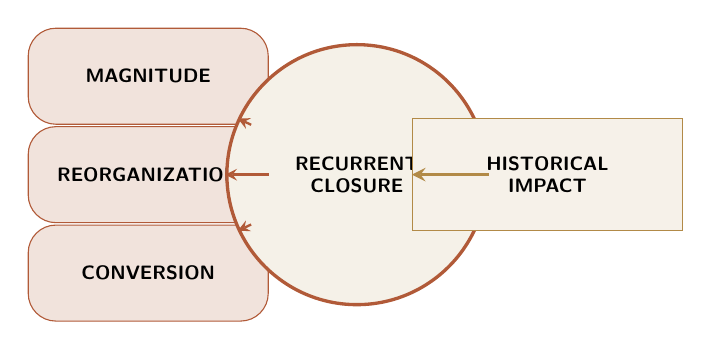
\begin{tikzpicture}[every node/.style={align=center}]
  \node[draw=Regulatory,fill=PaleRegulatory,rounded corners=10pt,minimum width=1.2in,minimum height=.48in,font=\sffamily\bfseries\scriptsize] (m) at (-1.65,1.25) {MAGNITUDE};
  \node[draw=Regulatory,fill=PaleRegulatory,rounded corners=10pt,minimum width=1.2in,minimum height=.48in,font=\sffamily\bfseries\scriptsize] (r) at (-1.65,0) {REORGANIZATION};
  \node[draw=Regulatory,fill=PaleRegulatory,rounded corners=10pt,minimum width=1.2in,minimum height=.48in,font=\sffamily\bfseries\scriptsize] (c) at (-1.65,-1.25) {CONVERSION};
  \node[circle,draw=Regulatory,line width=1.2pt,fill=Paper,minimum size=1.30in,font=\sffamily\bfseries\scriptsize] (gate) at (1.0,0) {RECURRENT\\CLOSURE};
  \node[draw=Gold,fill=Gold!12,minimum width=1.35in,minimum height=.56in,font=\sffamily\bfseries\scriptsize] (impact) at (3.42,0) {HISTORICAL\\IMPACT};
  \draw[-stealth,Regulatory,line width=.85pt] (m)--(gate);
  \draw[-stealth,Regulatory,line width=.85pt] (r)--(gate);
  \draw[-stealth,Regulatory,line width=.85pt] (c)--(gate);
  \draw[-stealth,Gold,line width=1.15pt] (gate)--(impact);
\end{tikzpicture}

\vspace{0.28in}
\begin{minipage}{0.82\linewidth}
\centering\itshape\fontsize{12.4}{17}\selectfont
Divergence creates reachable possibility. Recurrent closure converts possibility into history.
\end{minipage}
\end{center}
\vfill

\movementthree

\papersection{X}{The Singularity as a Civilizational Phase Transition}

The conventional singularity asks: \emph{When will artificial intelligence cross a capability threshold?}

The polymathic singularity asks: \emph{When does recursive coupling among humans, machines, institutions, and culture cause the entire selection landscape to reorganize?}

The transition includes:

\subhead{Biological inversion}
Previously maladaptive regulatory and attentional profiles acquire new niches and leverage.

\subhead{Educational inversion}
Static knowledge transmission loses relative value as adaptive learning, model-building, synthesis, and tool use rise.

\subhead{Economic inversion}
The cost of implementation falls while the value of judgment, framing, integration, trust, and direction rises.

\subhead{Institutional inversion}
Large organizations lose portions of their coordination advantage as individuals and small teams gain machine-mediated execution capacity.

\subhead{Epistemic inversion}
Knowing the correct stored answer becomes less valuable than asking the correct question, validating an answer, and connecting it to the wider system.

\subhead{Creative inversion}
Production ceases to be the primary bottleneck. Selection, coherence, taste, meaning, and integration become scarcer.

\subhead{Identity inversion}
The person previously described as unfocused because they crossed too many boundaries may become valuable precisely because the boundaries themselves no longer remain stable.

\pullquote{The singularity occurs not when AI awakens in isolation, but when recursively coupled intelligence makes the old organization of human capacity economically, educationally, and culturally unstable.}

This is the event horizon.

\papersection{XI}{Testable Predictions}

A theory of this scale must produce consequences that could fail.

\subhead{1. Environment-sensitive performance inversion}

Individuals with high novelty seeking, cross-domain interest, variable attention, or exoregulatory dependence should show disproportionate performance improvements in responsive, AI-rich, project-based environments compared with repetitive, delayed-feedback environments.

The predicted variable is not diagnosis alone. It is the interaction $\text{phenotype}\times\text{environment}$.

\subhead{2. AI should benefit integrative profiles differently}

AI assistance should produce especially large gains where users possess strong judgment, ideation, systems integration, or domain transfer but face bottlenecks in execution, organization, or technical translation.

\subhead{3. Unbounded AI coupling should destabilize some of the same users}

Without closure constraints, high-exoregulatory users should be unusually vulnerable to branch proliferation, compulsive iteration, sleep displacement, objective drift, unfinished artifacts, and stimulation replacing progress.

The same coupling channel should therefore generate both amplification and destabilization depending upon architecture. Research already indicates that generative AI can increase the evaluated creativity of individual outputs while reducing collective diversity, demonstrating that amplification at one scale can produce contraction at another.\sourcecue{SCIENCE}

\subhead{4. Educational advantage should migrate}

Project-based, interdisciplinary, adaptive, tool-mediated learning should increasingly outperform purely standardized instruction on tasks requiring transfer, synthesis, innovation, and real-world construction.

\subhead{5. Portfolios should gain relative power over credentials}

As individuals become able to produce cross-domain artifacts directly, demonstrated output should become more informative than static proxies of ability in a growing class of occupations.

\subhead{6. The specialist does not disappear}

Pure polymathy should not outperform deep specialization on every task. The predicted winner is a new arrangement:

\begin{equationpanel}
\begin{equation*}
\text{integrative orchestrators}+\text{deep specialists}+\text{AI execution layers}
\end{equation*}
\end{equationpanel}

\subhead{7. Social pathology labels should shift with economic demand}

Traits framed negatively under one labor regime should receive more favorable language as their economic value rises, even before their underlying biology changes.

\subhead{8. The phase transition should be uneven}

Regions, organizations, classes, and individuals with better access to AI, autonomy, education, capital, and social networks should experience the inversion earlier. The transition may initially widen inequality before new institutions catch up.

\papersection{XII}{The Working Thesis}

Human cognitive phenotypes vary in the degree to which they achieve allostatic and cognitive closure through internally sustained regulation versus active external coupling. Hunter and Farmer patterns may be higher-order ecological renderings of this deeper regulatory continuum. Agricultural, industrial, educational, and bureaucratic environments disproportionately rewarded internally stabilized, temporally standardized, specialized profiles while imposing substantial costs upon profiles dependent on novelty, movement, immediate feedback, cross-domain sampling, and environmental transformation.

The contemporary environment is entering a critical inversion driven by interacting technological, economic, cultural, educational, and institutional variables. Rising volatility, information velocity, cross-domain complexity, and cognitive externalization increasingly reward rapid adaptation, systems integration, ideational breadth, and tool-mediated execution.

Artificial intelligence is not the singular cause of this transition. It is an emergent artifact, coupling surface, environmental accelerator, conversion mechanism, and recursive feedback variable within it. By reducing the cost of translating thought into implementation, AI increases the leverage of integrative minds, accelerates the environment they are adapted to navigate, and changes the cultural selection pressures governing which phenotypes become economically productive and historically legible.

The resulting transition may constitute a polymathic singularity: a civilizational phase change in which the dominant unit of adaptive cognition shifts from the standardized linear specialist toward networks of externally coupled polymathic orchestrators, deep specialists, and machine intelligence.

\papersection{XIII}{Final Declaration}

\begin{center}
\begin{minipage}{0.90\linewidth}
\setlength{\parskip}{0.72em}
{\fontsize{13.3}{18}\selectfont
The old world selected for the person who could remain stable while the environment stayed fixed.

The emerging world increasingly selects for the person who can remain coherent while the environment transforms.

\textcolor{Polymathic}{\textbf{That is the inversion.}}

The polymath is not returning because knowledge has become smaller.

The polymath is returning because intelligence has become networked.

The specialist inherited a world of bounded problems.

The polymathic orchestrator is arriving because the boundaries are dissolving.

Artificial intelligence did not independently summon this world. Humanity built AI from inside an accelerating cultural transition, then placed it back into the environment as a recursive extension of cognition. The artifact now feeds into the minds, institutions, markets, and selection pressures that produced it.

The loop closes.\\
The environment rotates.\\
The suppressed phenotype becomes legible.\\
The latent ceiling acquires a conversion surface.

And what appeared to be the age of artificial intelligence reveals itself as something larger.}
\end{minipage}
\end{center}

\vfill
\begin{center}
{\color{Polymathic}\rule{1.0in}{2.5pt}}\\[0.22in]
{\sffamily\bfseries\fontsize{15}{19}\selectfont\letterspace{45}
THE AGE OF RECURSIVELY COUPLED INTELLIGENCE\\[0.12in]
\textcolor{Regulatory}{THE GREAT REGULATORY INVERSION}\\[0.12in]
\textcolor{Polymathic}{THE POLYMATHIC SINGULARITY}}
\end{center}

\clearpage
\thispagestyle{empty}
\begin{tikzpicture}[remember picture,overlay]
  \fill[Industrial] (current page.north west) rectangle (current page.south east);
  \coordinate (finalhub) at ([xshift=1.18in,yshift=-.62in]current page.center);
  \draw[Regulatory,opacity=.48,line width=1.2pt] (finalhub) circle (1.02in);
  \draw[Paper!35,opacity=.48,line width=.45pt] (finalhub) circle (.68in);
  \foreach \a in {0,40,...,320}{
    \coordinate (q\a) at ($(finalhub)+(\a:1.55in)$);
    \draw[Polymathic!65,opacity=.35,line width=.4pt] (finalhub)--(q\a);
    \fill[Paper!75,opacity=.75] (q\a) circle (1.8pt);
  }
  \fill[Gold,opacity=.80] (finalhub) circle (4pt);
\end{tikzpicture}
\vspace*{1.1in}
{\sffamily\bfseries\fontsize{9}{11}\selectfont\letterspace{180}\textcolor{Gold}{THE RESEARCH PROGRAM}}\par
\vspace{0.3in}
{\sffamily\bfseries\fontsize{25}{29}\selectfont\textcolor{Paper}{EARNING THE\\EVENT HORIZON}}\par
\vspace{0.28in}
\begin{minipage}{0.83\linewidth}
{\fontsize{11.2}{16}\selectfont\color{Paper!90}
This draft names a mechanism, a selection inversion, and a set of predictions large enough to reorganize how the transition is seen. Its next life is not about domesticating that claim. It is about making the claim measurable without making it small: resolving the literature, operationalizing regulatory closure bias, distinguishing metaphor from mechanism, and designing tests capable of proving the inversion wrong.

The ambition is already visible. The research program is how it earns the event horizon.}
\end{minipage}

\vfill
{\sffamily\fontsize{8}{11}\selectfont\color{Paper!60}
SOURCE-CUE KEY\\[0.12in]
PMC: PubMed Central \;\textbullet\; RSP: Royal Society Publishing \;\textbullet\; CUP: Cambridge University Press\\
JSTOR: JSTOR \;\textbullet\; HG: Harvard Gazette \;\textbullet\; OECD: OECD \;\textbullet\; UL: University of Louisville repository\\
SCIENCE: Science / associated research report\\[0.18in]
These labels reproduce the evidentiary resolution of the supplied draft. They are not complete references.}

\vspace{0.35in}
{\sffamily\bfseries\fontsize{8}{10}\selectfont\letterspace{90}\textcolor{Gold}{E.T. ELLIS \; / \; WORKING DRAFT v0.1}}

\end{document}
